\documentclass[letterpaper]{article}
\usepackage[margin=1in]{geometry}
\usepackage{times}
\usepackage{hyperref}
\usepackage{enumitem}
\usepackage{graphicx}
\usepackage{amssymb}


\title{\textbf{Bayesian Network Modeling of NFL Game Stats and Market Signals for Value Identification}}

\author{
  Leland Weeks\\
  \texttt{lhw22@drexel.edu}
  \and
  Johnny Belichev\\
  \texttt{jb4458@drexel.edu}
  \and
  Ishant Somal\\
  \texttt{is488@drexel.edu}
}

\date{May 3, 2026}

\begin{document}

\maketitle


\section{Problem Statement and Motivation}

The problem we are trying to solve is: Does partially overlapping information sources encode independent predictive information? For this problem, the domain and data we've chosen is game stats and market signals for NFL games.

Our motivation is to uncover whether line movement (market signals) contains information beyond game stats that reveal whether market pricing is efficient or not. Full efficiency would mean that there are no market signals or game stats that encode information not encoded by both together. If additional information exists in game stats that is not encoded within market signals, then there is information that could be exploited to further move the line towards efficiency. 

Our dataset spans 3,990 games over 15 seasons with 6 market data points per game including opening and closing spreads. The two data sources are joined by season and matchup (home and away teams). Our game stats data is from nflverse\cite{nflverse} and our market data is from SportsBookReviewsOnline.com\cite{sbr}. Sports betting markets have changed substantially since our data window - particularly following the 2018 repeal of PASPA, which legalized sports betting across U.S. states and dramatically increased market participation. The patterns identified in this study reflect a specific historical period and are not intended as a prescriptive betting system.


\begin{table}[ht]
	\centering
	\small
	\caption{Sample rows from \texttt{nfl\_game\_stats\_raw} (nflverse)}
	\begin{tabular}{llllrrrrr}
		\hline
		\textbf{Season} & \textbf{Wk} & \textbf{Home} & \textbf{Away} & \textbf{H Score} & \textbf{A Score} & \textbf{H EPA/play} & \textbf{H TOs} & \textbf{A TOs} \\
		\hline
		2007 & 1 & IND & NO  & 41 & 10 &  0.055 & 1 & 3 \\
		2007 & 1 & BUF & DEN & 14 & 15 & -0.074 & 1 & 1 \\
		2007 & 1 & CLE & PIT &  7 & 34 & -0.331 & 5 & 1 \\
		2007 & 1 & GB  & PHI & 16 & 13 & -0.082 & 4 & 1 \\
		2007 & 1 & HOU & KC  & 20 &  3 &  0.011 & 3 & 3 \\
		\hline
	\end{tabular}
	\label{tab:nflverse}
\end{table}


\begin{table}[ht]
	\centering
	\small
	\caption{Sample rows from \texttt{sbr\_nfl\_odds\_raw} (SBR)}
	\begin{tabular}{llllrrrrrr}
		\hline
		\textbf{Season} & \textbf{Home} & \textbf{Visitor} & \textbf{Open Sprd} & \textbf{Close Sprd} & \textbf{Open Tot} & \textbf{Close Tot} & \textbf{ML Home} & \textbf{ML Away} \\
		\hline
		2007-08 & Indianapolis   & NewOrleans  &  5.5 &  5.5 & 50.5 & 52.5 & -240 &  200 \\
		2007-08 & HoustonTexans  & KansasCity  & 38.5 &  3.0 &  0.0 & 37.5 & -200 &  170 \\
		2007-08 & Buffalo        & Denver      &  3.0 &  3.0 & 37.0 & 38.5 &  150 & -170 \\
		2007-08 & Cleveland      & Pittsburgh  &  4.5 &  5.0 & 37.5 & 36.0 &  195 & -235 \\
		2007-08 & Jacksonville   & Tennessee   &  6.5 &  7.5 & 37.5 & 39.5 & -350 &  290 \\
		\hline
	\end{tabular}
	\label{tab:sbr}
\end{table}

\section{Approach}

We plan to implement a Bayesian Network (BN) to test our hypothesis. The DAG structure shown in Figure~\ref{fig:dag} is a representation of our assumptions from the domain - historical stats drive the opening line, and the market reacts. Our BN will formally test conditional independence, specifically the causal relationship between line movement and game outcome. 

Our baseline will be Naive Bayes (NB) with assumption that all features are independent. We will use Hill Climbing as the main algorithm to encode our BN model, and we will use Peter-Clark (PC) as a validation check of the dependencies of our current DAG structure. We will test stats and market data in isolation and in combination. Comparing these three tests will tell us whether stats or market data is adding any signal or if they are redundant. If our BN can't beat Naive Bayes, then it means that the conditional dependencies  we're modeling don't provide predictive value, which will formally confirm that closing lines are efficient. 

Our dataset is dense with signal. First, the EPA per play is the most dense stat in football because it accounts for down, distance, and field position. Other stats, such as yards, turnovers, and scoring efficiency are highly correlated with EPA per play. We will also be able to derive a rolling average of Against-The-Spread (ATS) to substitute the actual ATS - because including the actual ATS would result in data leakage. Derivation of a rolling average ATS will be computed from previous games up to but not including the current game.

\begin{figure}[h!]
	\centering
	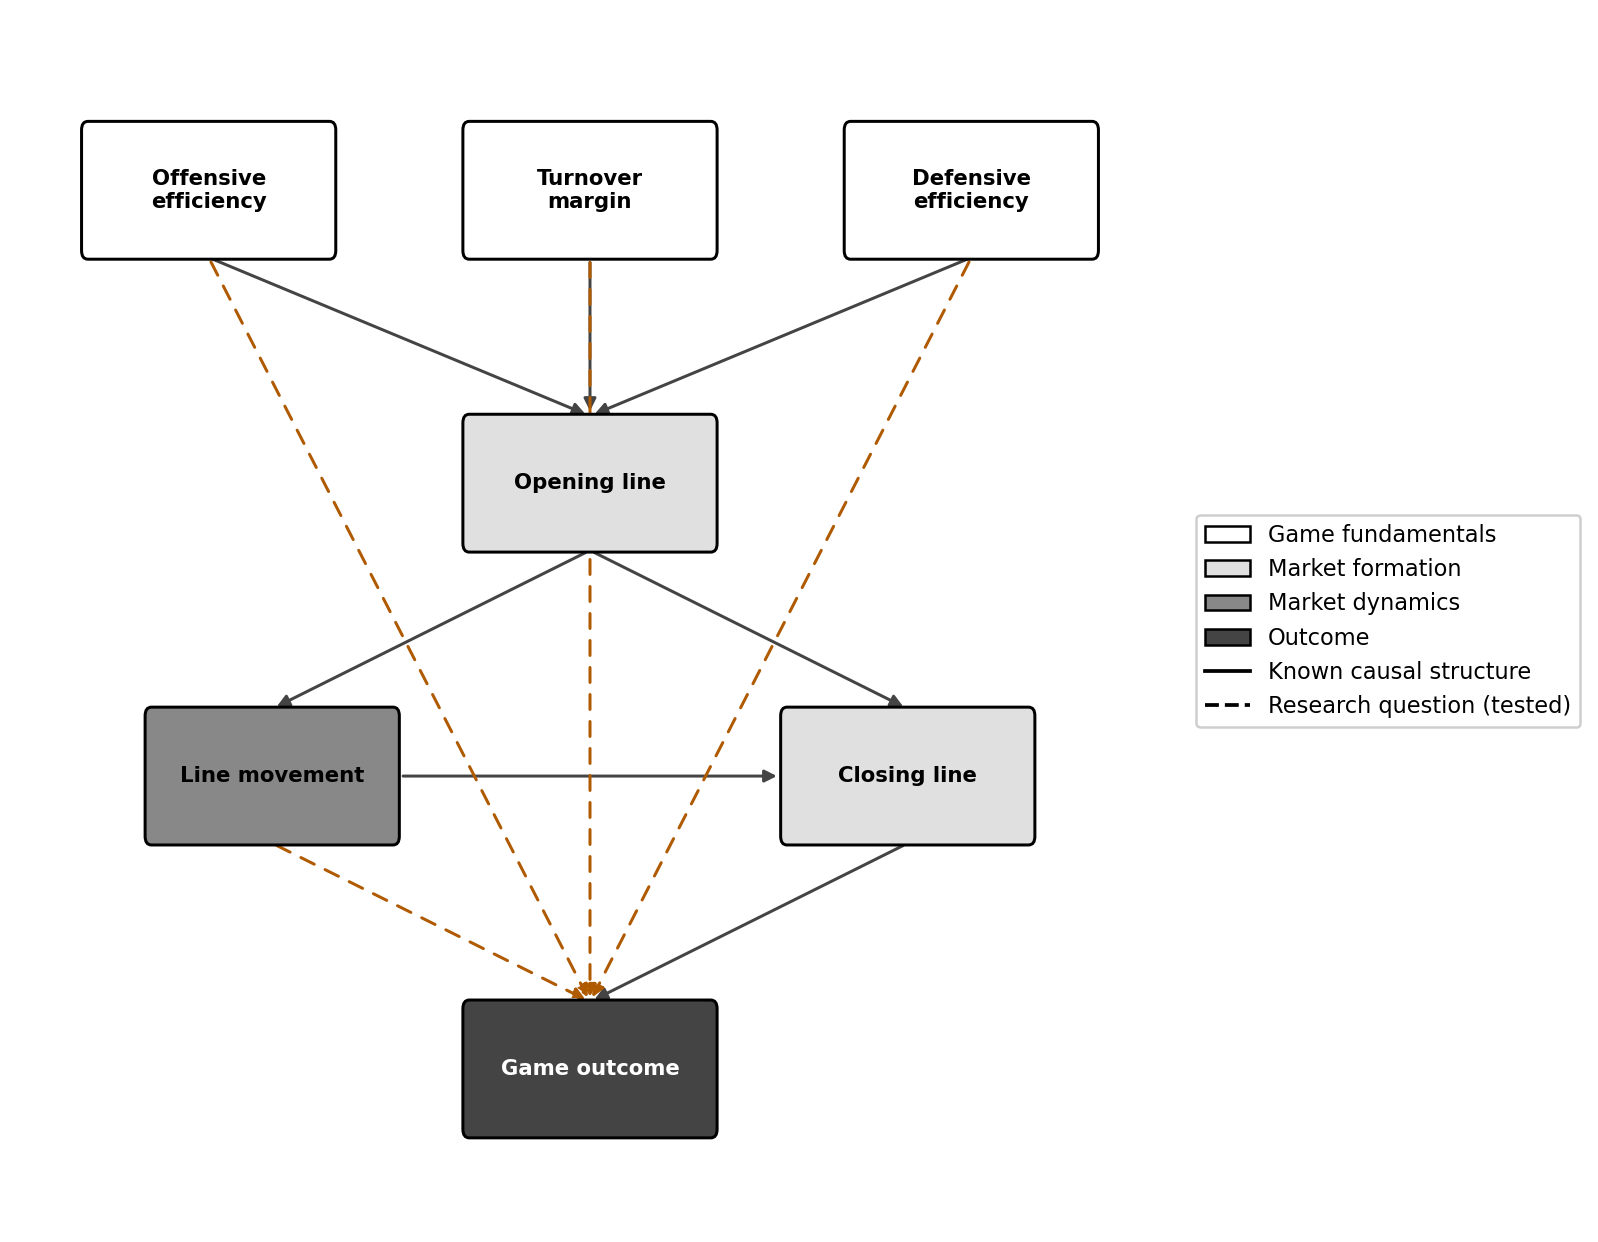
\includegraphics[width=0.7\linewidth]{approach_dag.png}
	\caption{Bayesian network DAG structure. Dashed arrows represent 
	hypothesized direct effects on game outcome — most critically, 
	whether line movement predicts outcome independent of game fundamentals.}	
	\label{fig:dag}
\end{figure}


\section{Related Work and Novelty}

Prior work has shown that probabilistic graphical models can be useful for sports prediction. Constantinou, Fenton, and Neil developed Bayesian network models for association football forecasting, showing that BNs can represent uncertain relationships between team strength, form, subjective factors, and match outcomes [3], [4]. However, their models focus mainly on game-related variables rather than modeling betting market movement as its own source of information. Other work has combined historical performance data with bookmaker odds. Egidi, Pauli, and Torelli use a hierarchical Bayesian model that blends historical team data with betting odds [5], while Hubáček, Šourek, and Železný study machine-learning systems that compare model predictions against bookmaker odds [6]. These studies show that market information can be useful, but they do not model the conditional dependence structure between game statistics, opening lines, line movement, and outcomes using a Bayesian network.

Separate research has studied betting market efficiency and line movement directly. Simon analyzes real-time betting line movement and finds that betting markets are mostly reliable but not always efficient [7]. Moskowitz studies sports betting as a market for detecting mispricing and momentum [8], while Szalkowski and Nelson examine NFL opening and closing lines as predictors of game outcomes [9]. Our project differs from these works by combining both perspectives: we use a Bayesian network to model game statistics and line movement together. The goal is not only to predict outcomes, but to test whether line movement contains additional predictive information after conditioning on game fundamentals. This makes the project a study of information overlap, conditional dependence, and market efficiency in NFL game pricing.


\section{Evaluation Approach}

For our three-class classification problem (cover / loss / push) with continuous features, we expect to start with the Gaussian Naive Bayes variant. We plan to compare stats-only, market-only, and combined models to test independent signal from the line movement. We plan to evaluate for predictive performance, calibration, and efficiency using Accuracy, Log Loss, and Brier Score. We may experiment with binary metrics, such as AUC-ROC, using a one-vs-rest approach.

\section{Milestones}

\begin{table}[h]
	\centering
	\small
	\caption{Project Milestones}
\begin{tabular}{l p{8cm} l}
		\hline
		\textbf{Due} & \textbf{Milestone} & \textbf{Owner} \\
		\hline
		Apr 26 & Data pipeline complete (acquisition + preprocessing)      & Done \\
		May 3  & Project Proposal submitted                          & Done \\
		May 7  & Proposal Presentation                               & All \\
		May 14 & DAG validation via PC algorithm                     & TBD \\
		May 17 & Naive Bayes baseline implemented and evaluated      & TBD \\
		May 21 & BN with Hill Climbing implemented                   & TBD \\
		May 24 & Ablation runs (stats only / market only / combined) & TBD \\
		May 26 & Results interpreted and written up                  & TBD \\
		May 28 & Paper draft complete                                & All \\
		May 31 & Final revisions and artifact submitted              & All \\
		Jun 4  & Final Presentation                                  & All \\
		\hline
	\end{tabular}
	\label{tab:milestones}
\end{table}


\begin{thebibliography}{9}

\bibitem{nflverse}
nflverse. 
\textit{nflverse: NFL data and R/Python packages for football analytics. https://nflverse.nflverse.com}.

\bibitem{sbr}
SportsBookReviewsOnline. 
\textit{NFL Odds Archives / Scores and Odds Archives. https://sportsbookreviewsonline.com/scoresoddsarchives/nfl/nfloddsarchives.htm}.

\bibitem{constantinou2012}
A. C. Constantinou, N. E. Fenton, and M. Neil, 
``pi-football: A Bayesian network model for forecasting Association Football match outcomes,'' 
\textit{Knowledge-Based Systems}, vol. 36, 2012. 
doi: 10.1016/j.knosys.2012.07.008.

\bibitem{constantinou2013}
A. C. Constantinou, N. E. Fenton, and M. Neil, 
``Profiting from an inefficient Association Football gambling market: Prediction, risk and uncertainty using Bayesian networks,'' 
\textit{Knowledge-Based Systems}, vol. 50, 2013. 
doi: 10.1016/j.knosys.2013.05.008.

\bibitem{egidi2018}
L. Egidi, F. Pauli, and N. Torelli, 
``Combining historical data and bookmakers' odds in modelling football scores,'' 
\textit{Statistical Modelling}, vol. 18, no. 5--6, 2018. 
doi: 10.1177/1471082X18798414.

\bibitem{hubacek2019}
O. Hubáček, G. Šourek, and F. Železný, 
``Exploiting sports-betting market using machine learning,'' 
\textit{International Journal of Forecasting}, vol. 35, no. 2, 2019. 
doi: 10.1016/j.ijforecast.2019.01.001.

\bibitem{simon2024}
J. Simon, 
``Inefficient forecasts at the sportsbook: An analysis of real-time betting line movement,'' 
\textit{Management Science}, vol. 70, no. 12, 2024. 
doi: 10.1287/mnsc.2022.00456.

\bibitem{moskowitz2021}
T. J. Moskowitz, 
``Asset Pricing and Sports Betting,'' 
\textit{The Journal of Finance}, vol. 76, no. 6, 2021. 
doi: 10.1111/jofi.13082.

\bibitem{szalkowski2012}
G. Szalkowski and M. L. Nelson, 
``The Performance of Betting Lines for Predicting the Outcome of NFL Games,'' 
\textit{arXiv preprint arXiv:1211.4000}, 2012.

\end{thebibliography}


\end{document}
